\documentclass[submit]{harvardml}

% Put in your full name and email address.
\name{Your Name}
\email{email@fas.harvard.edu}

% List any people you worked with.
\collaborators{%
  John Doe,
  Fred Doe
}

% You don't need to change these.
\course{CS181-S16}
\assignment{Assignment \#1}
\duedate{5:00pm February 5, 2016}

\usepackage[OT1]{fontenc}
\usepackage[colorlinks,citecolor=blue,urlcolor=blue]{hyperref}
\usepackage[pdftex]{graphicx}
\usepackage{subfig}
\usepackage{fullpage}
\usepackage{palatino}
\usepackage{mathpazo}
\usepackage{amsmath}
\usepackage{amssymb}
\usepackage{color}
\usepackage{todonotes}
\usepackage{listings}
\usepackage{common}

\usepackage[mmddyyyy,hhmmss]{datetime}

\definecolor{verbgray}{gray}{0.9}

\lstnewenvironment{csv}{%
  \lstset{backgroundcolor=\color{verbgray},
  frame=single,
  framerule=0pt,
  basicstyle=\ttfamily,
  columns=fullflexible}}{}


\begin{document}
\begin{center}
{\Large Homework 1: Linear Regression}\\
\end{center}
You should submit your answers as a PDF via the Canvas course website.  There is a mathematical component and a programming component to this homework.You may collaborate with others, but are expected to list collaborators, and write up your problem sets individually.\\

\noindent
Please type your solutions after the corresponding problems using this \LaTeX\ template, and start each problem on a new page.\\

%%%%%%%%%%%%%%%%%%%%%%%%%%%%%%%%%%%%%%%%%%%%%
% Problem 1
%%%%%%%%%%%%%%%%%%%%%%%%%%%%%%%%%%%%%%%%%%%%%
\begin{problem}[Centering and Ridge Regression, 7pts]
%\subsection*{1. Centering and Ridge Regression [7pts]}

Consider a data set in which each data input vector $\boldx \in \mathbb{R}^m$ is
centered, meaning $\forall \boldx, \sum_i x_i = 0$. Let $\boldX \in
\mathbb{R}^{n \times m}$ be the input matrix, the rows of which are the input
vectors. Let $\lambda$ be a positive constant. We define:

$$J(\boldw, w_0) = (\boldy - \boldX \boldw - w_0 {\bf 1 })^T (\boldy - \boldX
\boldw - w_0 {\bf 1 }) + \lambda \boldw^T \boldw$$

\begin{itemize}
  \item[(a)] Compute the gradient of $J(\boldw, w_0)$ with respect to $w_0$.
    Simplify as much as you can for full credit.
  \item[(b)] Compute the gradient of $J(\boldw, w_0)$ with respect to $\boldw$.
    Simplify as much as you can for full credit. Make sure to give your answer
    in matrix form.
  \item[(c)] Suppose that $\lambda > 0$. Knowing that $J$ is a convex function
    of its arguments, conclude that a global optimizer of
    $J(\boldw, w_0)$ is
    \begin{align}
      w_0 &= \frac{1}{n} \sum_i y_i \\
      \boldw &= (\boldX^T \boldX + \lambda \boldI)^{-1} \boldX^T \boldy
    \end{align}
    Before taking the inverse of a matrix, prove that it is invertible.
\end{itemize}
\end{problem}

\subsubsection*{Solution}











%%%%%%%%%%%%%%%%%%%%%%%%%%%%%%%%%%%%%%%%%%%%%
% Problem 2
%%%%%%%%%%%%%%%%%%%%%%%%%%%%%%%%%%%%%%%%%%%%%
\newpage
%\subsection*{2. Priors and Regularization [7pts]}
\begin{problem}[Priors and Regularization,7pts]
Consider the Bayesian linear regression model given in Bishop 3.3.1. The prior is
\begin{align*}
p(\boldw \given \alpha) = \mathcal{N}(\boldw \given \bold0, \alpha^{-1}\ident ),
\end{align*}
where $\alpha$ is the precision parameter that controls the variance of the Gaussian prior.  The likelihood can be written as
\begin{align*}
p(\boldt \given \boldw) &= \prod_{n=1}^N \mcN(t_n \given \boldw^\trans \bphi(\boldx_n), \beta^{-1}),
\end{align*}

Using the fact that the posterior is the product of the prior and the likelihood (up to a normalization constant), show that maximizing the log posterior (i.e., $\ln p(\boldw \given \boldt)= \ln p(\boldw | \alpha) + \ln p(\boldt \given \boldw)$) is equivalent to minimizing the regularized error term given by ${E_D(\boldw) + \lambda E_W(\boldw)}$ with 
\begin{align*}
E_D(\boldw) &= \frac{1}{2}\sum_{n = 1}^N (t_n - \boldw^\trans \bphi(\boldx_n))^2 \\
E_W(\boldw) &= \frac{1}{2}\boldw^\trans \boldw
\end{align*} 

Do this by writing $\ln p(\boldw \given \boldt)$ as a function of $E_D(\boldw)$ and $E_W(\boldw)$, dropping constant terms if necessary.  Conclude that maximizing this posterior is equivalent to minimizing the regularized error term given by $E_D(\boldw) + \lambda E_W(\boldw)$. (Hint: take $\lambda = \alpha/\beta$)
\end{problem}


\subsubsection*{Solution}



























%%%%%%%%%%%%%%%%%%%%%%%%%%%%%%%%%%%%%%%%%%%%%
% Problem 3
%%%%%%%%%%%%%%%%%%%%%%%%%%%%%%%%%%%%%%%%%%%%%
\newpage
\subsection*{3. Modeling Changes in Congress [10pts]}
 The objective of this problem is to learn about linear regression with basis
 functions by modeling the average age of the US Congress. The file
 \verb|congress-ages.csv| contains the data you will use for this problem.  It
 has two columns.  The first one is an integer that indicates the Congress
 number. Currently, the 114th Congress is in session. The second is the average
 age of that members of that Congress.  The data file looks like this:
\begin{csv}
congress,average_age
80,52.4959
81,52.6415
82,53.2328
83,53.1657
84,53.4142
85,54.1689
86,53.1581
87,53.5886
\end{csv}
and you can see a plot of the data in Figure~\ref{fig:congress}.

\begin{figure}[h]
\centering
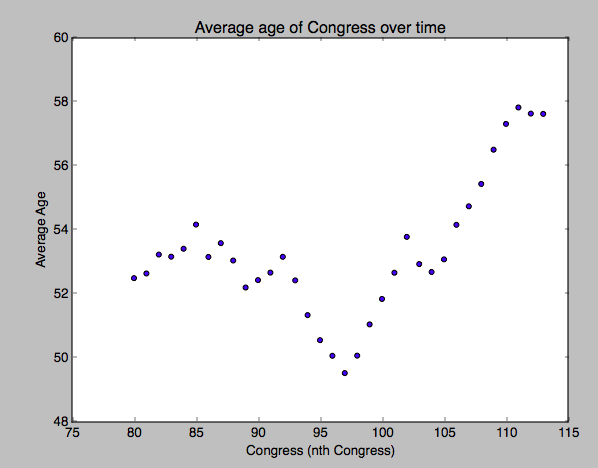
\includegraphics[width=0.8\textwidth]{congress-ages}
\caption{Average age of Congress.  The horizontal axis is the Congress number, and the vertical axis is the average age of the congressmen.}
\label{fig:congress}
\end{figure}

\begin{problem}[Modeling Changes in Congress, 10pts]
Implement basis function regression with ordinary least squares with the above
data. Some sample Python code is provided in \verb|linreg.py|, which implements
linear regression.  Plot the data and regression lines for the simple linear
case, and for each of the following sets of basis functions:
\begin{itemize}
	\item[(a)] $\phi_j(x) = x^j$ for $j=1, \ldots, 7$
	\item[(b)] $\phi_j(x) = x^j$ for $j=1, \ldots, 3$
	\item[(c)] $\phi_j(x) = \sin\{ x / j \}$ for $j=1, \ldots, 4$
	\item[(d)] $\phi_j(x) = \sin\{ x / j \}$ for $j=1, \ldots, 7$
	\item[(e)] $\phi_j(x) = \sin\{ x / j \}$ for $j=1, \ldots, 20$
\end{itemize}
  In addition to the plots, provide one or two sentences for each, explaining
  whether you think it is fitting well, overfitting or underfitting.  If it does
  not fit well, provide a sentence explaining why. A good fit should capture the
  most important trends in the data.
	\end{problem}

\subsubsection*{Solution}











\newpage
\begin{problem}[Calibration, 1pt]
Approximately how long did this homework take you to complete?
\end{problem}
\textbf{Answer:}

\end{document}
